\documentclass{beamer}
\usetheme[]{CambridgeUS}
%----macros begin-----------------------------------------------------------------------------------
\usepackage{graphicx}
\usepackage{color}
\usepackage{amsthm}

%\renewenvironment{Shaded}{\pause\begin{snugshade}}{\end{snugshade}}
\def\twocolumns#1#2{\begin{columns}
\begin{column}{0.5\linewidth}#1\end{column}
\begin{column}{0.5\linewidth}#2\end{column}
\end{columns}}
\def\mytwocolumns#1#2#3#4{\begin{columns}
\begin{column}{#1\linewidth}#2\end{column}
\begin{column}{#3\linewidth}#4\end{column}
\end{columns}}
\def\mythreecolumns#1#2#3#4#5#6{\begin{columns}
\begin{column}{#1\linewidth}#2\end{column}
\begin{column}{#3\linewidth}#4\end{column}
\begin{column}{#5\linewidth}#6\end{column}
\end{columns}}
\def\threecolumns#1#2#3{\begin{columns}
\begin{column}{0.33\linewidth}#1\end{column}
\begin{column}{0.33\linewidth}#2\end{column}
\begin{column}{0.33\linewidth}#3\end{column}
\end{columns}}
\def\fourcolumns#1#2#3#4{\begin{columns}%
\begin{column}{0.25\linewidth}#1\end{column}%
\begin{column}{0.25\linewidth}#2\end{column}%
\begin{column}{0.25\linewidth}#3\end{column}%
\begin{column}{0.25\linewidth}#4\end{column}%
\end{columns}}

\def\textbf#1{\alert{#1}}
\def\emph#1{{\color{cyan}#1}}
\def\conv{\mbox{\textrm{conv}\,}}
\def\aff{\mbox{\textrm{aff}\,}}
\def\E{\mathbb{E}}
\def\R{\mathbb{R}}
\def\Z{\mathbb{Z}}
\def\N{\mathbb{N}}
\def\v#1{{\bf #1}}
\def\p#1{{\bf #1}}
\def\T#1{{\bf #1}}
\def\vet#1{{\left(\begin{array}{cccccccccccccccccccc}#1\end{array}\right)}}
\def\mat#1{{\left(\begin{array}{cccccccccccccccccccc}#1\end{array}\right)}}

\def\lin{\mbox{\rm lin}\,}
\def\aff{\mbox{\rm aff}\,}
\def\pos{\mbox{\rm pos}\,}
\def\cone{\mbox{\rm cone}\,}
\def\conv{\mbox{\rm conv}\,}
\newcommand{\homog}[0]{\mbox{\rm homog}\,}
\newcommand{\relint}[0]{\mbox{\rm relint}\,}

%----macros end-----------------------------------------------------------------------------------

\newtheorem{remark}[theorem]{Remark}

% \usepackage{beamerthemesplit} // Activate for custom appearance

\title{Literate programming IDE for LARCC}
%\author{Till Tantau}
\date{\today}

\begin{document}

\frame{\titlepage}

\section[Outline]{}
\frame{\tableofcontents}

%///////////////////////////////////////////////////////////////////////////////
\section{Introduction}
%///////////////////////////////////////////////////////////////////////////////
%-------------------------------------------------------------------------------
\frame
{
  \frametitle{Introduction}
  \framesubtitle{Why this document was written}

Some ideas, links, and docs on how to write technical papers, including source programming codes, that anyone can understand and execute 

\vfill

This document was written to start documenting the implementation of the new software system entitled either 3C/LAR (to read as 'Compute with CoChains over LAR') or LAR4CCC (LAR for Compute with CoChains)

\vfill
BUT

\vfill
it may work well for \emph{any kind of scientific programming} \alert{including the computer code} and both \alert{the how} and \alert{the why} it works ... 

\emph{In any language} or combination of languages

}
%-------------------------------------------------------------------------------
\subsection{Literate Programming}
%-------------------------------------------------------------------------------
\frame
{
  \frametitle{Literate Programming}
  \framesubtitle{Donald Knuth. "Literate Programming (1984)" in Literate Programming. CSLI, 1992, pg. 99.}
  \footnotesize

\begin{columns}
	\begin{column}{6cm}
I believe that the time is ripe for significantly better documentation of programs, and that we can best achieve this by considering programs to be works of literature. Hence, my title: "Literate Programming."

Let us change our traditional attitude to the construction of programs: Instead of imagining that our main task is to instruct a computer what to do, let us concentrate rather on explaining to human beings what we want a computer to do.	
	\end{column}
\pause
	\begin{column}{6cm}
The practitioner of literate programming can be regarded as an essayist, whose main concern is with exposition and excellence of style. Such an author, with thesaurus in hand, chooses the names of variables carefully and explains what each variable means. He or she strives for a program that is comprehensible because its concepts have been introduced in an order that is best for human understanding, using a mixture of formal and informal methods that reinforce each other.	
	\end{column}
\end{columns}

}
%-------------------------------------------------------------------------------
%-------------------------------------------------------------------------------
\begin{frame}[fragile]
  \frametitle{Donald Knuth}
  \framesubtitle{The CWEB System of Structure Documentation. Addison-Wesley. 1994. pg. 1.}
  \footnotesize

\begin{columns}
	\begin{column}{4.5cm}
An experienced programmer, to provide the best possible documentation of software products, \emph{needs two things simultaneously}: \alert{a language like TeX} \emph{for formatting}, and \alert{a language like C} \emph{for programming}. 

\vspace{10mm}
Neither type of language can provide the best documentation by itself; but \emph{when both are appropriately combined}, we obtain a system that is much more useful than either language separately.	
	\end{column}
\pause\hspace{-0.5cm}
	\begin{column}{8cm}
\begin{itemize}
\item \href{http://www-cs-faculty.stanford.edu/~knuth/taocp.html}{\alert{The Art of Computer Programming}}

{\scriptsize
At the end of 1999, these books were named \emph{among the best twelve physical-science monographs of the century} by {\it American Scientist}, along with: Dirac on {\it quantum mechanics}, Einstein on {\it relativity}, Mandelbrot on {\it fractals}, Pauling on the {\it chemical bond}, Russell and Whitehead on {\it foundations of mathematics}, von Neumann and Morgenstern on {\it game theory}, Wiener on {\it cybernetics}, Woodward and Hoffmann on {\it orbital symmetry}, Feynman on {\it quantum electrodynamics}, Smith on the {\it search for structure}, and Einstein's {\it collected papers}
}

\item \href{http://www.amazon.com/Computers-Typesetting-Volumes-A-E-Boxed/dp/0201734168/ref=sr_1_1?ie=UTF8&qid=1385620263&sr=8-1}{\alert{Computers \& Typesetting}}

{\scriptsize
complete documentation of the TeX and METAFONT systems for digital typography.
%\footnote{\scriptsize
%\begin{minipage}[t]{5cm}
%Volumes A and C are hardcover versions of the paperback user manuals.
%Volumes B and D contain source code for TeX and METAFONT, respectively, written with literate
% programming methodology. 
%\end{minipage}
%}
``Never before has a computer program of this size been spelled out so clearly and completely.''
}

%\item  \href{http://www.amazon.com/Physically-Based-Rendering-Second-Edition/dp/0123750792}{\alert{Physically Based Rendering}, From Theory To Implementation}
\end{itemize}
	

	\end{column}
\end{columns}

\end{frame}
%-------------------------------------------------------------------------------
%-------------------------------------------------------------------------------
\frame
{
  \frametitle{Literate Programming resources}
  \framesubtitle{\href{http://www.literateprogramming.com/}{\emph{http://www.literateprogramming.com/}}}

\begin{columns}
	\begin{column}{5cm}
		\alert{Quotes}
		\begin{itemize}
			\item 
			Literate Programming
			\item 
			Software Documentation
			\item 
			Design Documentation
			\item 
			Agile Documentation
			\item 
			Source Code Comments
			\item 
			Software Aging
		\end{itemize}
	\end{column}
\pause
	\begin{column}{5cm}
		\alert{Category}
		\begin{itemize}
			\item 
			CWEB
			\item 
			Articles
			\item 
			Tools
			\item 
			Links
		\end{itemize}
		\alert{Community}
		\begin{itemize}
			\item 
			Feedback
		\end{itemize}
	\end{column}
\end{columns}


}
%-------------------------------------------------------------------------------
\subsection{Compute-with-Cochains over LAR}
%--------------------------------------------------------------------------------
\begin{frame}
\frametitle{Starting today !!} 
\framesubtitle{\bf Compute-with-CoChains over LAR software in development}


\begin{enumerate}
\item \alert{CAD-PLM Lab}, Dip. Matematica e Fisica, Univ Roma Tre 
\item \alert{Spatial Automation Lab}, Univ of Wisconsin at Madison
\item \alert{CEDMAV}, SCI Institute, Univ of Utah
\end{enumerate}

\vfill\pause
\alert{Integrated tools being used} (for now)

\begin{itemize}
\item \emph{GitHub} (social development)
\item \emph{Literate programming} (Latex + Leo + Nuweb)
\item \emph{Haskell} (as specification language)
\item \emph{Python \& PyOpenCL} (for rapid Prototyping)
\item \emph{Javascript \& WebCL} (for client-based web applications)
\item \emph{C++ \& OpenCL} (for optimized deployement)
\end{itemize}


\end{frame}
%-------------------------------------------------------------------------
%///////////////////////////////////////////////////////////////////////////////
\section{Software tools}
%///////////////////////////////////////////////////////////////////////////////
\subsection{\LaTeX}
%-------------------------------------------------------------------------------
\frame
{
  \frametitle{LaTeX --- A document preparation system}
  \framesubtitle{\href{http://latex-project.org/ftp.html}{\bf Obtaining LaTeX}}
  \footnotesize

\begin{columns}
	\begin{column}{6cm}
\begin{itemize}
\item 
\LaTeX\ is the \alert{de facto standard for} the communication and publication of \alert{scientific documents} 
\item 
It is a specialisation of \TeX, \emph{the highest-quality} typesetting system by D.~Knuth, and includes features designed for fast production of \emph{technical and scientific documentation} 
\item 
\LaTeX\ is available as \href{http://latex-project.org/ftp.html}{\emph{free software}}
\end{itemize}

\flushright
(from \href{http://www.latex-project.org/}{\emph{www.latex-project.org}})
	\end{column}
\pause
	\begin{column}{6cm}
	The \alert{\texttt{larcc} IDE} requires the users to embed the compute code within \LaTeX\ files written for documenting their work. Therefore the \alert{first requirement is a working \LaTeX\ environment} 
	
	\begin{remark}[For Windows users]
	``As \TeX\ Live is the basis of Mac\TeX, and is the \TeX\ system for Unix, if you work cross-platform and want an identical system on all of your machines, then \href{http://www.tug.org/texlive/}{\emph{\TeX\ Live}} is the way to go''.
	\end{remark}
	\end{column}
\end{columns}

}
%-------------------------------------------------------------------------------
\subsection{Leo}
%-------------------------------------------------------------------------------
\frame
{
  \frametitle{Leo editor}
  \framesubtitle{After the first experiments with literate programming I realised that any standard (linear) editor is not the best one for it. {\bf Then I found a wonderful non-linear editor}}
  \footnotesize

\begin{columns}
	\begin{column}{6cm}
\begin{remark}[What it is]
Leo is a \alert{PIM}, \alert{IDE} and \alert{outliner} that accelerates the work-flow of programmers, authors and web designers
\end{remark}

\vspace{5mm}

"Leo is the best IDE that I have had the pleasure to use. It has totally changed not only the way that I program, but also the way that I store and organize all of the information that I need for the job that I do."―Ian Mulvany
	\end{column}
\pause
	\begin{column}{6cm}
\begin{remark}[Leo features]
\begin{itemize}
\item 
\emph{Leo outlines} are views on an underlying \alert{graph} (DAG)
\item 
Outline \emph{nodes} can \alert{reside in many places} within a single outline.
\item 
\emph{Outline-oriented markup} generates \alert{external files} from outlines.
\end{itemize}
\end{remark}

\vspace{3mm}
\href{http://leoeditor.com/tutorial.html}{\emph{Learn about Leo in two hours}}


	\end{column}
\end{columns}

\centering\vfill
download: \href{http://leoeditor.com/}{\alert{http://leoeditor.com/}}

}
%-------------------------------------------------------------------------------
\subsection{Nuweb}
%-------------------------------------------------------------------------------
\begin{frame}[fragile]

  \frametitle{Multi-language literate programming}
  \framesubtitle{The simplest incarnation of the Knut's original work}
  \footnotesize

\begin{columns}

	\begin{column}{6cm}
\alert{Nuweb} works with any \emph{programming language and \LaTeX}, and is probably the simplest incarnation of the Knut's original work.

The web site of the tool is \href{http://sourceforge.net/projects/nuweb/}{\emph{sourceforge.net/projects/nuweb/}}

A revised version of source files:\\ 
\href{https://code.google.com/p/nuweb/downloads/list}{\alert{code.google.com/p/nuweb}}	
	\end{column}
	
\pause	

	\begin{column}{6cm}
This package can build using the standard tools:
\begin{verbatim}
$ cd <path-to>/nuweb/
$ ./configure
$ make
$ sudo make install
\end{verbatim}
For some documentation read the \href{https://code.google.com/p/nuweb/source/browse/branches/qse-nuweb/README?r=3}{wiki} page.  Test your installation by just compiling to \emph{pdf} the \texttt{nuweb.w} document itself, whose chapter one contains the user documentation:
\begin{verbatim}
$ nuweb nuweb.w
\end{verbatim}	
	\end{column}
\end{columns}

\vfill
\alert{User manual} (first chapter of compiled \texttt{nuweb.w}): \href{run:nuwebdoc.pdf}{\emph{nuwebdoc.pdf}}

\end{frame}
%-------------------------------------------------------------------------------
\frame
{
  \frametitle{Nuweb example 1/2}
  \framesubtitle{Sorgente \LaTeX\ con marcatura \texttt{Nuweb}}

   \centering
   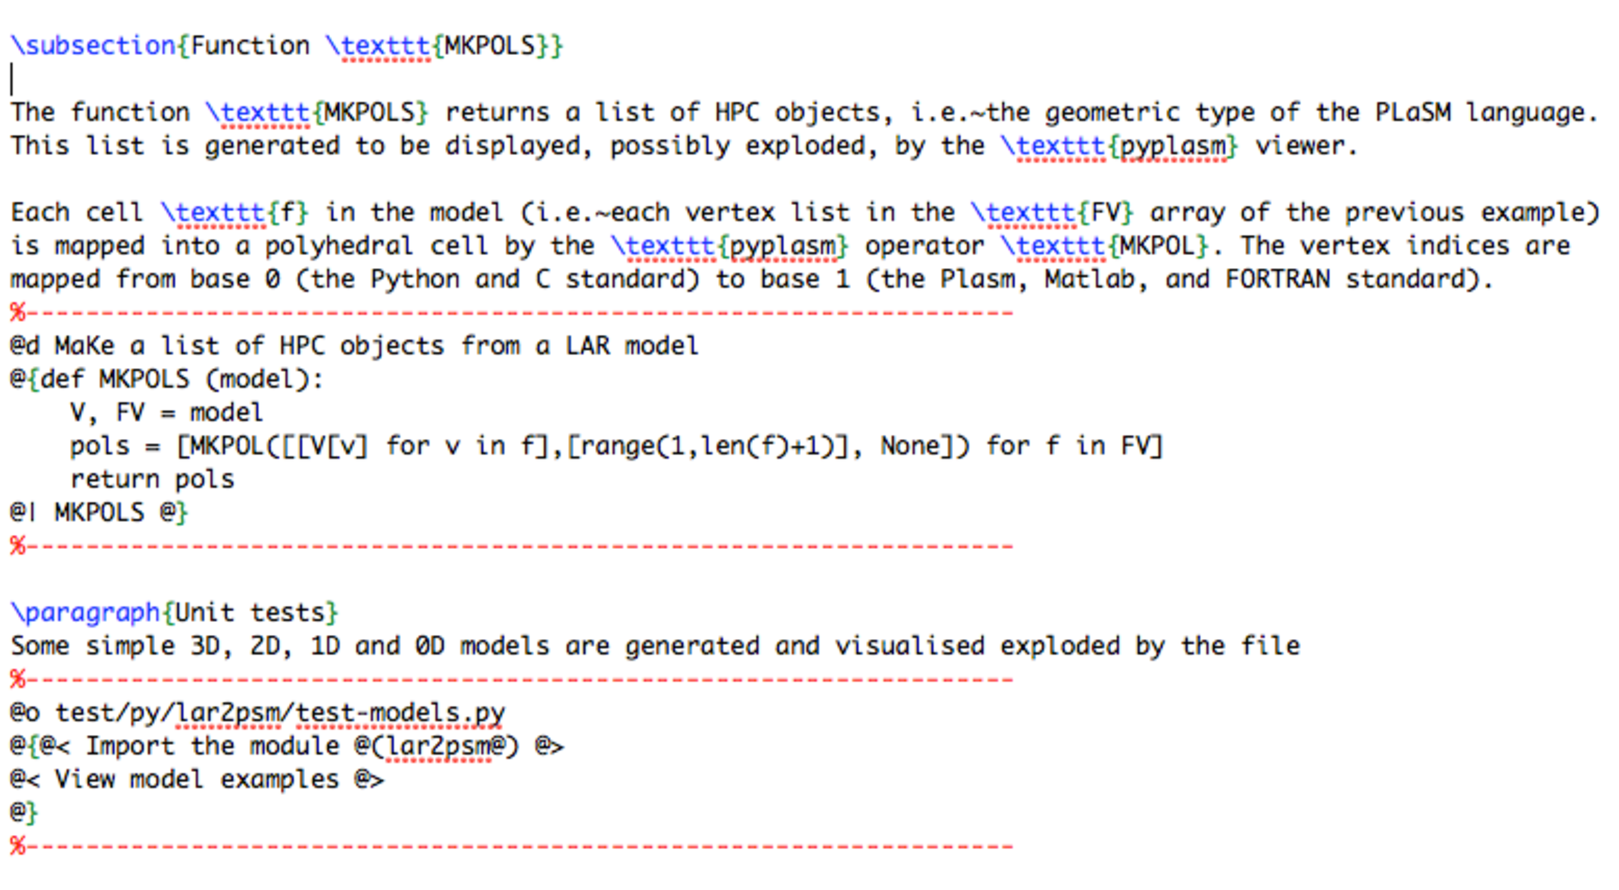
\includegraphics[width=\linewidth]{figs/nuweb1} 

}
%-------------------------------------------------------------------------------
%-------------------------------------------------------------------------------
\frame
{
  \frametitle{Nuweb example 2/2}
  \framesubtitle{compilato \texttt{pdf}}

   \centering
   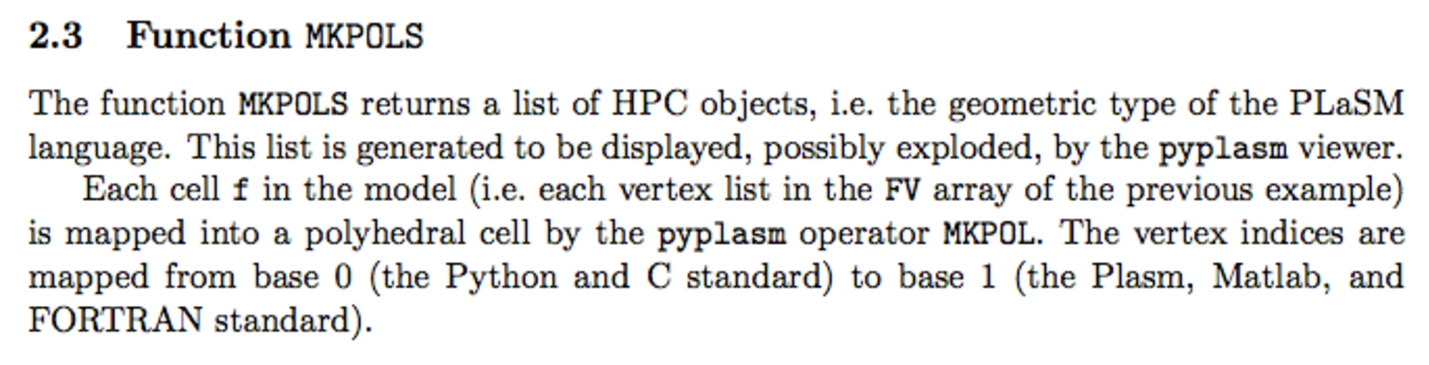
\includegraphics[width=0.8\linewidth]{figs/nuweb2} 
   
   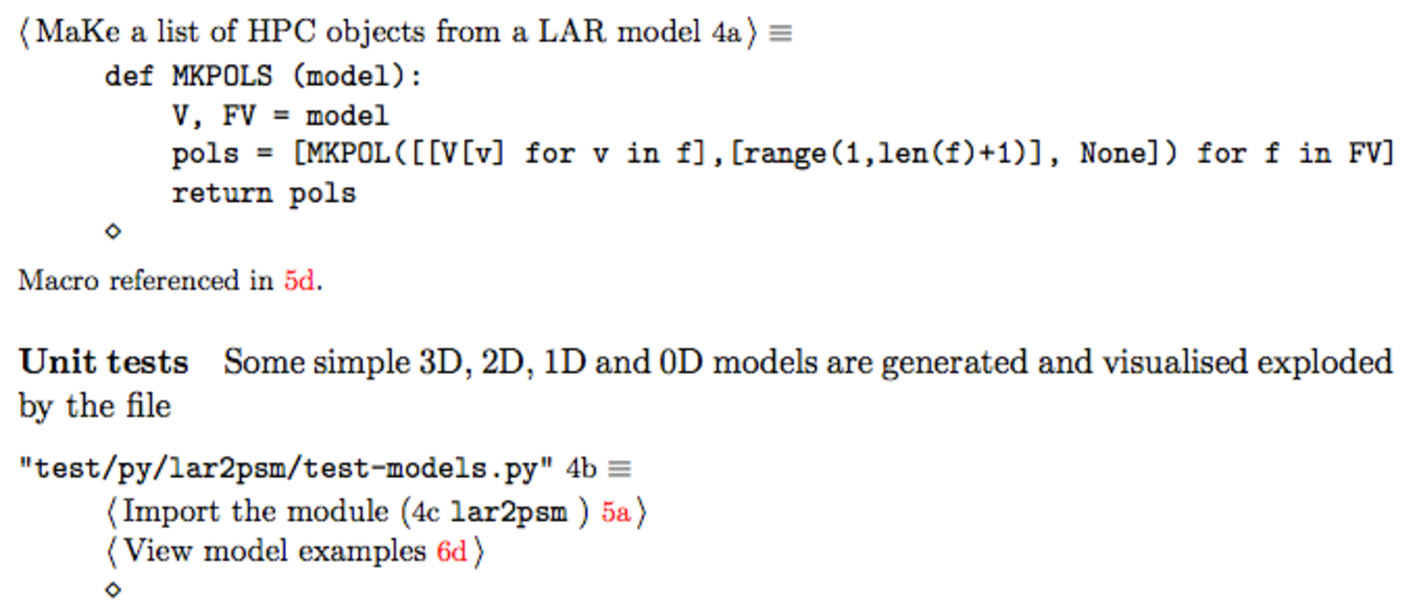
\includegraphics[width=0.8\linewidth]{figs/nuweb3} 

}
%-------------------------------------------------------------------------------
%-------------------------------------------------------------------------------
\subsection{Makefile}
%-------------------------------------------------------------------------------
\begin{frame}[fragile]
  \frametitle{Make utility}
  \framesubtitle{Just few words ...}

\begin{columns}
	\begin{column}{6cm}
In software development, \alert{Make is a utility} that \emph{automatically builds executable programs and libraries from source code} by reading files called \alert{makefiles} which specify how to derive the target program. 
	\end{column}
\pause
	\begin{column}{6cm}
\emph{Make is invoked} with a list of \alert{target} file names to build as command-line arguments:
\begin{verbatim}
    $ make [TARGET ...]
\end{verbatim}
Without arguments, Make builds the first target that appears in its makefile, which is traditionally a target named \emph{all}	
	\end{column}
\end{columns}

\end{frame}
%-------------------------------------------------------------------------------
%-------------------------------------------------------------------------------
\begin{frame}[fragile]
  \frametitle{Makefile short tutorial (wikipedia)}
  \footnotesize

\begin{itemize}
\item 
\alert{A makefile consists of rules}. Each rule begins with a \emph{textual dependency line} which defines a \alert{target} followed by a colon (:) and \emph{optionally an enumeration of components} (files or other targets) \emph{on which the target depends} 

\item 
It is common to refer to components as \alert{prerequisites} of the target.

\item 
Usually each rule has a \alert{single unique target}, rather than multiple targets.

\item[]
   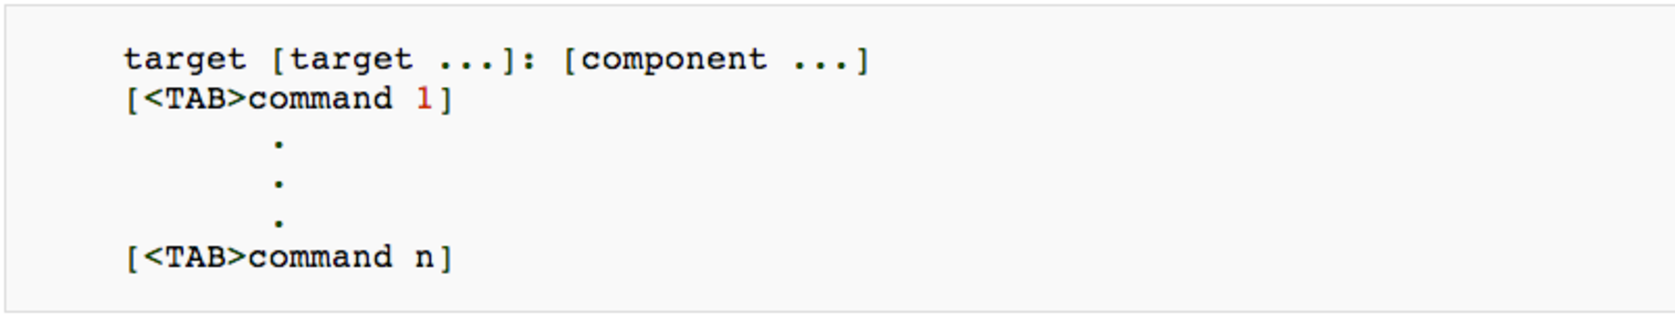
\includegraphics[width=0.8\linewidth]{figs/makefile} 

\item 
After each dependency line, a \emph{series of command lines} may follow which define \alert{how to transform the components (usually source files) into the target (usually the "output")}. If \emph{any of the components have been modified}, the command lines are run.

\item 
Each \emph{command line} must begin with a \alert{tab character} to be recognized as a command. 
\end{itemize}


\end{frame}
%-------------------------------------------------------------------------------
%-------------------------------------------------------------------------------
\begin{frame}[allowframebreaks,fragile]
  \frametitle{The (current) Makefile for \texttt{larcc} ---}
  \tiny
\begin{verbatim}
#
# Makefile for cclar
#

NAME = lar2psm
LANGUAGE = py
BIBFILE = $(NAME).bib

IDIR = src/tex/
ODIR = lib/
DOCTEX = doc/tex/
DOCPDF = doc/pdf/

all: 
    echo building $(NAME)
    make pdf
    make clear
    open $(DOCPDF)$(NAME).pdf

exec:
    cp $(IDIR)macros.tex macros.tex
    cp $(IDIR)bib.bib $(BIBFILE)
    cp -R $(IDIR)images . 
    cp $(IDIR)$(NAME).tex $(NAME).w
    
    nuweb $(NAME).w

pdf: $(IDIR)$(NAME).tex
    make exec
    
    pdflatex $(NAME).tex
    nuweb $(NAME)
    bibtex $(NAME)
    
    pdflatex $(NAME).tex
    pdflatex $(NAME).tex

html:
    make pdf
    
    rm -dfR $(NAME)/*
    rm -dfR $(NAME)
    mkdir $(NAME)
    cp src/html/css.cfg $(NAME).cfg
    makeindex $(NAME).tex
    htlatex $(NAME).tex "$(NAME).cfg,TocLink,html,index=2,3"
    mv -fv images $(NAME).html $(NAME).css $(NAME)
    rm -fv $(NAME).* macros.tex
    mv -fv $(NAME)*.* $(NAME)
    if [ -d doc/html/$(NAME) ] ; then rm -R doc/html/$(NAME) ; fi
    mv $(NAME) doc/html/
    open doc/html/$(NAME)/$(NAME).html

tests:
    echo `python test/py/test01.py`
    echo `python test/py/test02.py`
    echo `python test/py/test06.py`


clear:
    mv -fv $(NAME).tex $(NAME).bbl macros.tex $(DOCTEX)
    mv -fv $(NAME).pdf $(DOCPDF)
    mv -fv $(NAME).w $(ODIR)w
    if [ -d $(DOCTEX)images ] ; then rm -R $(DOCTEX)images ; fi
    mv -fv images $(DOCTEX)
    rm $(NAME).*
\end{verbatim}

\end{frame}
%-------------------------------------------------------------------------------
\subsection{GitHub}
%-------------------------------------------------------------------------------
\begin{frame}[fragile]
  \frametitle{Git \& GitHub}
  \framesubtitle{{\bf Git} \emph{the tool}, {\bf GitHub} \emph{the service} for projects that uses Git}

Every \emph{Git working directory} is a full-fledged \alert{repository} with complete history and \emph{full \alert{version tracking} capabilities}, not dependent on network access or a central server

\vfill

\begin{columns}
	\begin{column}{6.5cm}
\begin{itemize}
\item 
Put your IDE under the protection of a \alert{version control system}. 

\item 
\emph{\texttt{larcc}} comes from \href{https://github.com/}{\alert{Github}} equipped with an \emph{integrated Git} 
\end{itemize}
	\end{column}
\pause
	\begin{column}{6cm}
\begin{itemize}
\item 
\emph{Mac OS X}: \alert{\texttt{Git}} available by default.
\item 
\emph{Else}: download and install
\href{http://git-scm.com/downloads}{\alert{http://git-scm.com/downloads}}
\end{itemize}
	\end{column}
\end{columns}

\vfill

\begin{remark}[\alert{To download \texttt{larcc}}]
\begin{verbatim}
$ git clone https://github.com/cvdlab/larcc
\end{verbatim}
\end{remark}

\end{frame}
%-------------------------------------------------------------------------------
%-------------------------------------------------------------------------------
%///////////////////////////////////////////////////////////////////////////////
\section{Up and Running}
%///////////////////////////////////////////////////////////////////////////////
%-------------------------------------------------------------------------------
\frame
{
  \frametitle{aaaaaaaaaa}
  \framesubtitle{bbbbbb}

\begin{columns}
	\begin{column}{6cm}
	
	\end{column}
\pause
	\begin{column}{6cm}
	
	\end{column}
\end{columns}

}
%-------------------------------------------------------------------------------
%-------------------------------------------------------------------------------
\frame
{
  \frametitle{aaaaaaaaaa}
  \framesubtitle{bbbbbb}

\begin{columns}
	\begin{column}{6cm}
	
	\end{column}
\pause
	\begin{column}{6cm}
	
	\end{column}
\end{columns}

}
%-------------------------------------------------------------------------------
%-------------------------------------------------------------------------------
\frame
{
  \frametitle{aaaaaaaaaa}
  \framesubtitle{bbbbbb}

\begin{columns}
	\begin{column}{6cm}
	
	\end{column}
\pause
	\begin{column}{6cm}
	
	\end{column}
\end{columns}

}
%-------------------------------------------------------------------------------
%-------------------------------------------------------------------------------
\frame
{
  \frametitle{aaaaaaaaaa}
  \framesubtitle{bbbbbb}

\begin{columns}
	\begin{column}{6cm}
	
	\end{column}
\pause
	\begin{column}{6cm}
	
	\end{column}
\end{columns}

}
%-------------------------------------------------------------------------------
%-------------------------------------------------------------------------------
\frame
{
  \frametitle{aaaaaaaaaa}
  \framesubtitle{bbbbbb}

\begin{columns}
	\begin{column}{6cm}
	
	\end{column}
\pause
	\begin{column}{6cm}
	
	\end{column}
\end{columns}

}
%-------------------------------------------------------------------------------
%-------------------------------------------------------------------------------
\frame
{
  \frametitle{aaaaaaaaaa}
  \framesubtitle{bbbbbb}

\begin{columns}
	\begin{column}{6cm}
	
	\end{column}
\pause
	\begin{column}{6cm}
	
	\end{column}
\end{columns}

}
%-------------------------------------------------------------------------------
%///////////////////////////////////////////////////////////////////////////////
\section{Structure of LARCC}
%///////////////////////////////////////////////////////////////////////////////
%-------------------------------------------------------------------------------
\frame
{
  \frametitle{aaaaaaaaaa}
  \framesubtitle{bbbbbb}

\begin{columns}
	\begin{column}{6cm}
	
	\end{column}
\pause
	\begin{column}{6cm}
	
	\end{column}
\end{columns}

}
%-------------------------------------------------------------------------------
%-------------------------------------------------------------------------------
\frame
{
  \frametitle{aaaaaaaaaa}
  \framesubtitle{bbbbbb}

\begin{columns}
	\begin{column}{6cm}
	
	\end{column}
\pause
	\begin{column}{6cm}
	
	\end{column}
\end{columns}

}
%-------------------------------------------------------------------------------
%-------------------------------------------------------------------------------
\frame
{
  \frametitle{aaaaaaaaaa}
  \framesubtitle{bbbbbb}

\begin{columns}
	\begin{column}{6cm}
	
	\end{column}
\pause
	\begin{column}{6cm}
	
	\end{column}
\end{columns}

}
%-------------------------------------------------------------------------------
%-------------------------------------------------------------------------------
\frame
{
  \frametitle{aaaaaaaaaa}
  \framesubtitle{bbbbbb}

\begin{columns}
	\begin{column}{6cm}
	
	\end{column}
\pause
	\begin{column}{6cm}
	
	\end{column}
\end{columns}

}
%-------------------------------------------------------------------------------
%-------------------------------------------------------------------------------
\frame
{
  \frametitle{aaaaaaaaaa}
  \framesubtitle{bbbbbb}

\begin{columns}
	\begin{column}{6cm}
	
	\end{column}
\pause
	\begin{column}{6cm}
	
	\end{column}
\end{columns}

}
%-------------------------------------------------------------------------------
%-------------------------------------------------------------------------------
\frame
{
  \frametitle{aaaaaaaaaa}
  \framesubtitle{bbbbbb}

\begin{columns}
	\begin{column}{6cm}
	
	\end{column}
\pause
	\begin{column}{6cm}
	
	\end{column}
\end{columns}

}
%-------------------------------------------------------------------------------
\end{document}
